%
% main.tex -- Paper zum Thema <bessel>
%
% (c) 2026 Gian Cavegn, OST Ostschweizer Fachhochschule
%
% !TEX root = ../../buch.tex
% !TEX encoding = UTF-8
% !TeX spellcheck = de_CH
%
\chapter{Bessel-Funktionen\label{chapter:bessel}}
\kopflinks{Bessel-Funktionen}
\begin{refsection}
\chapterauthor{Gian Cavegn}
 
%
% Reihenfolge der Abschnitte
%
%   teil0  Einleitung
%   teil1  Herleitung der Bessel-Differentialgleichung
%   teil2  Lösung mit verallgemeinerten Potenzreihen
%   teil3  Eigenschaften der Bessel-Funktionen
%   teil4  Modifizierte Bessel-Funktionen I_nu und K_nu
%   teil5  Anwendung, die Kepler-Gleichung vlt?
%
%

%
% teil0.tex -- Einleitung
%
% (c) 2026 Gian Cavegn, OST Ostschweizer Fachhochschule
%
% !TEX root = ../../buch.tex
% !TEX encoding = UTF-8
% !TeX spellcheck = de_CH
%
\section{Einleitung\label{bessel:section:einleitung}}
\kopfrechts{Einleitung}
%
% Aufgabe dieses Abschnitts.
% Den Leser abholen, motivieren, ankündigen.
% Eine bis anderthalb Seiten, keine Unterabschnitte.
% Zuletzt schreiben -- die Einleitung verspricht, was das Kapitel hält.
%
Eine gespannte Saite und ein Trommelfell gehorchen derselben Wellengleichung.
Trotzdem klingt eine Saite harmonisch und eine Trommel nicht.
Der Grund dafür liegt nicht in der Physik, sondern in der Geometrie.
Die Saite ist eindimensional, die Membran ist kreisförmig.
Sobald man die Wellengleichung in Polarkoordinaten schreibt und den winkelabhängigen Anteil abspaltet, bleibt für den radialen Anteil eine gewöhnliche Differentialgleichung zweiter Ordnung übrig, deren Lösungen nicht mehr die vertrauten Sinus- und Kosinusfunktionen sind.
Diese Lösungen sind die Bessel-Funktionen.

Bessel-Funktionen treten überall dort auf, wo ein Problem rotationssymmetrisch ist.
Die Schwingungen einer kreisförmigen Membran gehören dazu, ebenso die Wärmeleitung in einem Zylinder, die Beugung von Licht an einer runden Blende und die Ausbreitung von Wellen in einem Rohr.
Sie sind damit für die Kreisgeometrie das, was Sinus und Kosinus für die Gerade sind.

Ihren Namen tragen sie nach Friedrich Wilhelm Bessel (1784--1846), der sie 1824 systematisch untersuchte \cite{bessel:bessel1824}.
Bemerkenswert ist, dass Bessel dabei überhaupt nicht von einem Schwingungsproblem ausging, sondern von der Himmelsmechanik.
Er suchte eine Reihenentwicklung für die Lösung der Kepler-Gleichung, also für die Position eines Planeten auf seiner Ellipsenbahn als Funktion der Zeit.
Einzelne Funktionen dieser Familie waren allerdings schon lange vorher aufgetaucht.
Daniel Bernoulli stiess bei der Untersuchung der schwingenden Kette auf diejenige Funktion, die wir heute $J_0$ nennen; seine Arbeit erschien im Band der Petersburger \emph{Commentarii} für die Jahre 1732/33, der allerdings erst 1738 gedruckt wurde \cite{bessel:bernoulli1732}.
Euler behandelte die schwingende kreisförmige Membran und gelangte dabei zur Differentialgleichung selbst, ebenfalls in einem Band für das Jahr 1764, der erst zwei Jahre später erschien \cite{bessel:euler1764}.
Noch früher, in einem Brief an Leibniz vom 3.~Oktober 1703, hatte Jakob Bernoulli eine Reihe angegeben, die sich rückblickend als Bessel-Funktion der Ordnung $\frac13$ lesen lässt \cite{bessel:dutka1995}.
Erst Bessel hat die Funktionen dieser Familie als Ganzes untersucht und ihre Eigenschaften systematisch zusammengetragen.
Beide Zugänge, der schwingungstheoretische und der himmelsmechanische, kommen in diesem Kapitel vor.

Das Kapitel schliesst unmittelbar an Kapitel~\ref{chapter:differentialgleichungen} an.
Dort wurde gezeigt, dass sich Lösungen einer Differentialgleichung mit analytischen Koeffizienten als Potenzreihe ansetzen lassen, und im Abschnitt über die fuchssche Differentialgleichung wurde dieser Ansatz auf verallgemeinerte Potenzreihen ausgedehnt.
Genau dieser erweiterte Ansatz wird hier gebraucht.
% teil0, Z. 42
Die Bessel-Gleichung hat im Ursprung eine Singularität.
Ein gewöhnlicher Potenzreihenansatz liefert dort für nicht ganzzahlige Ordnung nur die triviale Lösung und für ganzzahlige Ordnung nie die zweite Lösung.
Die Bessel-Funktionen sind also nicht nur ein weiteres Beispiel für die Theorie aus Kapitel~\ref{chapter:differentialgleichungen}, sondern gewissermassen deren Musterbeispiel.
An ihnen lässt sich ablesen, wozu der Aufwand mit dem zusätzlichen Exponenten $\varrho$ überhaupt betrieben wurde.

Der Aufbau ist der folgende.
Abschnitt~\ref{bessel:section:herleitung} leitet die Bessel-Differentialgleichung aus der Wellengleichung einer kreisförmigen Membran her und macht dabei sichtbar, an welcher Stelle die Rotationssymmetrie ins Spiel kommt.
Abschnitt~\ref{bessel:section:loesung} löst diese Gleichung mit dem Ansatz aus Kapitel~\ref{chapter:differentialgleichungen} und liefert die Bessel-Funktionen erster und Art.
Abschnitt~\ref{bessel:section:eigenschaften} stellt die Eigenschaften zusammen, die für das Rechnen mit diesen Funktionen nötig sind, also Rekursionsformeln, Nullstellen, Orthogonalität und asymptotisches Verhalten.
Abschnitt~\ref{bessel:section:modifiziert} behandelt die modifizierten Bessel-Funktionen, die bei rein imaginärem Argument entstehen.
% Die beiden letzten Abschnitte zeigen die Theorie in Aktion, einmal an der Lichtbeugung am Kreisspalt (Abschnitt~\ref{bessel:section:lichtbeugung}) und einmal an der Kepler-Gleichung (Abschnitt~\ref{bessel:section:kepler}), also an genau jenem Problem, das Bessel ursprünglich zu diesen Funktionen geführt hat.
%
% teil1.tex -- Herleitung der Bessel-Differentialgleichung
%
% (c) 2026 Gian Cavegn, OST Ostschweizer Fachhochschule
%
% !TEX root = ../../buch.tex
% !TEX encoding = UTF-8
% !TeX spellcheck = de_CH
%
\section{Herleitung der Bessel-Differentialgleichung
\label{bessel:section:herleitung}}
\kopfrechts{Herleitung}
%
% Ziel dieses Abschnitts.
% Zeigen, dass die Bessel-DGL nicht vom Himmel fällt, sondern
% zwangsläufig entsteht, sobald man ein Wellenproblem auf einem
% Kreisgebiet separiert.
% Roter Faden, Rechteck -> Kreis. Am Rechteck geht alles mit sin/cos
% auf, am Kreis nicht mehr.
%
Die Bessel-Differentialgleichung fällt nicht vom Himmel.
Sie entsteht zwangsläufig, sobald man ein Schwingungsproblem auf einem kreisförmigen Gebiet in Koordinaten zerlegt, die zur Geometrie passen.
Dieser Abschnitt führt die Rechnung von der Wellengleichung bis zur fertigen Differentialgleichung durch.
%
% Die schwingende Membran
%
\subsection{Die schwingende Membran
\label{bessel:herleitung:subsection:membran}}
Eine eingespannte Membran wird durch ihre Auslenkung $u(x,y,t)$ senkrecht zur Ruhelage beschrieben.
Für kleine Auslenkungen genügt $u$ der Wellengleichung
\begin{equation}
\frac{\partial^2 u}{\partial t^2}
=
c^2 \Delta u,
\qquad
\Delta
=
\frac{\partial^2}{\partial x^2}
+
\frac{\partial^2}{\partial y^2},
\label{bessel:herleitung:eqn:welle}
\end{equation}
wobei $c$ die Ausbreitungsgeschwindigkeit ist.
Die Wellengleichung~\eqref{bessel:herleitung:eqn:welle} ergibt sich aus einer Kraftbilanz am Flächenelement.
Die Membran habe die Flächendichte $\mu$ und stehe unter der homogenen Spannung $\sigma$, gemessen als Kraft pro Länge.
An jeder Kante eines Rechtecks mit den Kantenlängen $dx$ und $dy$ zieht die Spannung tangential an der Membran.
Für kleine Auslenkungen ist die vertikale Komponente dieser Kraft proportional zur Steigung, für die beiden Kanten senkrecht zur $x$-Achse also
\[
\sigma\,dy
\bigl(
u_x(x+dx,y) - u_x(x,y)
\bigr)
\approx
\sigma\, u_{xx}\, dx\, dy .
\]
Der Beitrag der beiden anderen Kanten ist $\sigma u_{yy}\,dx\,dy$.
Das zweite Newtonsche Gesetz liefert damit
\[
\mu\, dx\, dy\; u_{tt}
=
\sigma \bigl( u_{xx} + u_{yy} \bigr) dx\, dy ,
\]
und Division durch $\mu\,dx\,dy$ ergibt \eqref{bessel:herleitung:eqn:welle} mit $c^2 = \sigma/\mu$.
Vorausgesetzt sind dabei kleine Auslenkungen, eine über die ganze Membran konstante Spannung und eine verschwindende Biegesteifigkeit.
Eine ausführliche Herleitung findet sich bei \cite{bessel:courant}.
Am Rand der Membran ist die Auslenkung null, es gilt also $u=0$ auf dem Rand des Gebietes.
Für die Zeitabhängigkeit macht man den Separationsansatz
\begin{equation}
u(x,y,t)
=
T(t)\, v(x,y).
\label{bessel:herleitung:eqn:zeitsep}
\end{equation}
Einsetzen in~\eqref{bessel:herleitung:eqn:welle} und Division durch
$c^2Tv$ ergibt
\[
\frac{1}{c^2}\frac{T''(t)}{T(t)}
=
\frac{\Delta v(x,y)}{v(x,y)}.
\]
Die linke Seite hängt nur von $t$ ab, die rechte nur von $x$ und $y$.
Beide Seiten müssen daher konstant sein.
Nennt man diese Konstante $-k^2$, so zerfällt das Problem in die harmonische Schwingungsgleichung $T''=-c^2k^2T$ und in die
\emph{Helmholtz-Gleichung}
\index{Helmholtz-Gleichung}%
\begin{equation}
\Delta v + k^2 v = 0.
\label{bessel:herleitung:eqn:helmholtz}
\end{equation}
Die zeitliche Abhängigkeit ist damit erledigt, sie ist immer sinusförmig mit der Kreisfrequenz $\omega = ck$.
Die ganze Information über die Form der Membran steckt in
\eqref{bessel:herleitung:eqn:helmholtz}.
%
% Rechteck und Kreis
%
\subsection{Rechteck und Kreis
\label{bessel:herleitung:subsection:rechteckkreis}}
An dieser Stelle lohnt sich ein Vergleich, der zeigt, wo die Schwierigkeit liegt.
 
Für eine rechteckige Membran mit den Seitenlängen $a$ und $b$ führt der Ansatz $v(x,y)=X(x)Y(y)$ auf die beiden Gleichungen
$X''=-\alpha^2X$ und $Y''=-\beta^2Y$ mit $\alpha^2+\beta^2=k^2$.
Beide sind Schwingungsgleichungen mit konstanten Koeffizienten, ihre Lösungen sind Sinus- und Kosinusfunktionen, und die Randbedingungen liefern
\[
v_{mn}(x,y)
=
\sin\frac{m\pi x}{a}
\sin\frac{n\pi y}{b},
\qquad
m,n \in \mathbb{N}.
\]
Das Problem ist mit den Funktionen der elementaren Analysis vollständig gelöst.
 
Bei einer kreisförmigen Membran versagt dieser Ansatz.
Der Rand ist ein Kreis, und in kartesischen Koordinaten lässt sich die Randbedingung nicht in eine Bedingung an $X$ und eine an $Y$ zerlegen.
Man muss Koordinaten wählen, in denen der Rand eine Koordinatenfläche ist, und das sind die Polarkoordinaten.
Der Preis dafür ist, dass der Laplace-Operator in diesen Koordinaten nicht mehr konstante Koeffizienten hat.
Genau daraus entsteht die Bessel-Gleichung.
%
% Separation in Polarkoordinaten
%
\subsection{Separation in Polarkoordinaten
\label{bessel:herleitung:subsection:polar}}
In Polarkoordinaten $x=r\cos\varphi$, $y=r\sin\varphi$ lautet der Laplace-Operator
\begin{equation}
\Delta
=
\frac{\partial^2}{\partial r^2}
+
\frac{1}{r}\frac{\partial}{\partial r}
+
\frac{1}{r^2}\frac{\partial^2}{\partial\varphi^2}.
\label{bessel:herleitung:eqn:laplacepolar}
\end{equation}
Diese Form erhält man mit der Kettenregel aus $r=\sqrt{x^2+y^2}$ und $\varphi=\arctan(y/x)$.
Wegen
\[
\frac{\partial r}{\partial x} = \cos\varphi,
\qquad
\frac{\partial r}{\partial y} = \sin\varphi,
\qquad
\frac{\partial\varphi}{\partial x} = -\frac{\sin\varphi}{r},
\qquad
\frac{\partial\varphi}{\partial y} = \frac{\cos\varphi}{r}
\]
lauten die Ableitungsoperatoren
\[
\frac{\partial}{\partial x}
=
\cos\varphi\,\frac{\partial}{\partial r}
-
\frac{\sin\varphi}{r}\,\frac{\partial}{\partial\varphi},
\qquad
\frac{\partial}{\partial y}
=
\sin\varphi\,\frac{\partial}{\partial r}
+
\frac{\cos\varphi}{r}\,\frac{\partial}{\partial\varphi}.
\]
Wendet man beide ein zweites Mal an und addiert, so heben sich die gemischten Ableitungen 
$\partial^2/\partial r\,\partial\varphi$ und die Terme mit $\partial/\partial\varphi$ paarweise weg, 
und mit $\cos^2\varphi+\sin^2\varphi=1$ bleibt\eqref{bessel:herleitung:eqn:laplacepolar} übrig.
Zu beachten ist dabei, dass die Koeffizienten $\cos\varphi$ und $\sin\varphi/r$ selbst von $r$ und $\varphi$ abhängen und deshalb mitdifferenziert werden müssen.
Genau daraus entsteht der Term $\frac{1}{r}\frac{\partial}{\partial r}$.
Die Helmholtz-Gleichung~\eqref{bessel:herleitung:eqn:helmholtz} wird damit zu
\begin{equation}
\frac{\partial^2 v}{\partial r^2}
+
\frac{1}{r}\frac{\partial v}{\partial r}
+
\frac{1}{r^2}\frac{\partial^2 v}{\partial\varphi^2}
+
k^2 v
=
0.
\label{bessel:herleitung:eqn:helmholtzpolar}
\end{equation}
Die Koeffizienten $1/r$ und $1/r^2$ sind der entscheidende Unterschied zum kartesischen Fall.
Sie sind bei $r=0$ singulär, und diese Singularität wird uns im nächsten Abschnitt wieder begegnen.
Nun separiert man ein zweites Mal, diesmal in Radius und Winkel,
\begin{equation}
v(r,\varphi)
=
R(r)\,\Phi(\varphi).
\label{bessel:herleitung:eqn:radialsep}
\end{equation}
Einsetzen in~\eqref{bessel:herleitung:eqn:helmholtzpolar} und Multiplikation mit $r^2/(R\Phi)$ ergibt
\[
\frac{r^2R''(r) + rR'(r) + k^2r^2R(r)}{R(r)}
=
-\frac{\Phi''(\varphi)}{\Phi(\varphi)}.
\]
Wieder hängt die linke Seite nur von $r$ ab und die rechte nur von $\varphi$, beide sind also konstant.
Wir nennen die Konstante $n^2$.
 
Für den Winkelanteil bleibt
\begin{equation}
\Phi''(\varphi) + n^2\Phi(\varphi) = 0
\label{bessel:herleitung:eqn:winkel}
\end{equation}
mit den Lösungen $\Phi(\varphi)=\cos n\varphi$ und $\Phi(\varphi)=\sin n\varphi$.
Hier kommt eine Bedingung ins Spiel, die es beim Rechteck nicht gibt.
Die Winkelkoordinate ist periodisch, es muss $\Phi(\varphi+2\pi)=\Phi(\varphi)$ gelten.
Daraus folgt $n\in\mathbb{Z}$.
Die Separationskonstante ist also nicht frei wählbar, sondern durch die Geometrie auf ganze Zahlen festgelegt.
 
%
% Die Bessel-Differentialgleichung
%
\subsection{Die Bessel-Differentialgleichung
\label{bessel:herleitung:subsection:besseldgl}}
Für den Radialanteil bleibt
\begin{equation}
r^2R''(r) + rR'(r) + (k^2r^2-n^2)R(r) = 0.
\label{bessel:herleitung:eqn:radial}
\end{equation}
Mit der Substitution $x=kr$ und $y(x)=R(x/k)$ verschwindet der
Parameter $k$, denn es ist
$R'(r)=k\,y'(x)$ und $R''(r)=k^2y''(x)$, und man erhält
\begin{equation}
x^2y''(x) + xy'(x) + (x^2-n^2)y(x) = 0.
\label{bessel:herleitung:eqn:bessel}
\end{equation}
Das ist die \emph{Bessel-Differentialgleichung}
\index{Bessel-Differentialgleichung}%
der Ordnung $n$.
 
Aus der Herleitung ergibt sich $n$ als ganze Zahl.
Die Gleichung~\eqref{bessel:herleitung:eqn:bessel} ist aber für jeden reellen oder komplexen Parameter sinnvoll, und die Lösungstheorie des nächsten Abschnitts braucht die Ganzzahligkeit an keiner Stelle.
Wir schreiben deshalb ab jetzt

\begin{equation}
x^2y'' + xy' + (x^2-\nu^2)y = 0,
\qquad
\nu \in \mathbb{R},\ \nu \ge 0,
\label{bessel:herleitung:eqn:besselnu}
\end{equation}
und nennen $\nu$ die \emph{Ordnung}
\index{Ordnung einer Bessel-Funktion}%
der Gleichung.
Halbzahlige Ordnungen treten zum Beispiel bei kugelsymmetrischen Problemen auf, wo dieselbe Rechnung in Kugelkoordinaten durchgeführt wird.
 
Ein Blick auf~\eqref{bessel:herleitung:eqn:besselnu} zeigt schon, wo die Schwierigkeit liegt.
Dividiert man durch $x^2$, so lautet die Gleichung
\[
y''
+
\frac{1}{x}y'
+
\frac{x^2-\nu^2}{x^2}y
=
0,
\]
und die Koeffizienten haben bei $x=0$ einen Pol.
Der Existenzsatz für Potenzreihenlösungen aus Kapitel~\ref{chapter:differentialgleichungen} ist daher nicht anwendbar.
Tatsächlich ergibt der Ansatz $y=\sum_k a_kx^k$ die Bedingung $(k^2-\nu^2)a_k=-a_{k-2}$, und für nicht ganzzahliges $\nu$ bleibt davon nur die triviale Lösung übrig.
Die Gleichung ist aber von genau der Bauart
\[
x^2y'' + p(x)\,xy' + q(x)\,y = 0
\]
mit den bei $0$ analytischen Funktionen $p(x)=1$ und $q(x)=x^2-\nu^2$, sie ist also eine fuchssche Differentialgleichung im Sinne von Abschnitt~\ref{buch:differentialgleichungen:section:fuchs}.
Damit steht das Werkzeug für ihre Lösung bereits zur Verfügung.
%
% teil2.tex -- Lösung mit verallgemeinerten Potenzreihen
%
% (c) 2026 Gian Cavegn, OST Ostschweizer Fachhochschule
%
\section{Lösung mit verallgemeinerten Potenzreihen
\label{bessel:section:loesung}}
\kopfrechts{Lösung}
%
% Ziel dieses Abschnitts.
% Die allgemeine Theorie aus dem Fuchs-Abschnitt nicht wiederholen,
% sondern anwenden.
% Der Mehrwert liegt darin, dass die Bessel-Gleichung ein besonders
% sauberer Spezialfall ist.
% Es gilt F(varrho) = varrho^2 - nu^2, also varrho = +- nu.
%
Die Bessel-Gleichung
\begin{equation}
x^2y'' + xy' + (x^2-\nu^2)y = 0
\label{bessel:loesung:eqn:bessel}
\end{equation}
ist eine fuchssche Differentialgleichung.
Das in Abschnitt~\ref{buch:differentialgleichungen:section:fuchs} entwickelte Verfahren lässt sich deshalb direkt anwenden.
Wir wiederholen die allgemeine Theorie hier nicht, sondern setzen ein und beobachten, was dabei herauskommt.
Bemerkenswert ist, wie einfach der Spezialfall wird.
Alle Grössen der allgemeinen Rekursion nehmen für die Bessel-Gleichung eine besonders übersichtliche Form an.
 
%
% Die Bessel-Gleichung als fuchssche Gleichung
%
\subsection{Die Bessel-Gleichung als fuchssche Gleichung
\label{bessel:loesung:subsection:fuchssch}}
Der Vergleich von~\eqref{bessel:loesung:eqn:bessel} mit der allgemeinen Form \eqref{buch:differentialgleichungen:fuchs:eqn:dgl} liefert
\begin{equation}
p(x) = 1,
\qquad
q(x) = x^2-\nu^2.
\label{bessel:loesung:eqn:pq}
\end{equation}
Beide Funktionen sind Polynome, ihre Potenzreihenentwicklungen um $0$ brechen also nach wenigen Gliedern ab.
Für die Koeffizienten $p_l$ und $q_l$ bedeutet das
\begin{equation}
p_0 = 1,
\quad
p_l = 0
\ \text{für}\ l \ge 1,
\qquad
q_0 = -\nu^2,
\quad
q_1 = 0,
\quad
q_2 = 1,
\quad
q_l = 0
\ \text{für}\ l\ge 3.
\label{bessel:loesung:eqn:koeffizienten}
\end{equation}
Der Ansatz ist eine verallgemeinerte Potenzreihe im Sinne der Definition~\ref{buch:differentialgleichungen:verallgemeinert:def}, also
\begin{equation}
y(x)
=
\sum_{k=0}^\infty
a_k x^{k+\varrho}
=
x^\varrho
\sum_{k=0}^\infty
a_k x^k,
\qquad
a_0 \ne 0.
\label{bessel:loesung:eqn:ansatz}
\end{equation}
Der Faktor $x^\varrho$ ist der ganze Unterschied zu einem gewöhnlichen Potenzreihenansatz.
Er ist genau das, was das Verfahren rettet, denn er erlaubt der Lösung, sich bei $x=0$ wie eine beliebige, auch nicht ganzzahlige Potenz zu verhalten.
 
%
% Indexgleichung
%
\subsection{Die Indexgleichung
\label{bessel:loesung:subsection:index}}
Die Indexgleichung des Fuchs-Verfahrens lautet $F(\varrho) = \varrho(\varrho-1) + \varrho p_0 + q_0 = 0$.
Mit den Werten~\eqref{bessel:loesung:eqn:koeffizienten} wird daraus
\begin{equation}
F(\varrho)
=
\varrho(\varrho-1) + \varrho - \nu^2
=
\varrho^2 - \nu^2.
\label{bessel:loesung:eqn:index}
\end{equation}
Die beiden linearen Terme heben sich weg, und es bleibt die denkbar einfachste quadratische Gleichung.
Ihre Lösungen sind
\begin{equation}
\varrho_1 = \nu,
\qquad
\varrho_2 = -\nu.
\label{bessel:loesung:eqn:varrho}
\end{equation}
Der Exponent der verallgemeinerten Potenzreihe ist also nichts anderes als die Ordnung der Gleichung, mit beiden Vorzeichen.
Das ist keine blosse Rechenkuriosität, sondern lässt sich direkt ablesen.
Für kleine $x$ ist der Term $x^2$ in~\eqref{bessel:loesung:eqn:bessel}
gegenüber $\nu^2$ vernachlässigbar, und die Gleichung geht in
\[
x^2y'' + xy' - \nu^2 y = 0
\]
über.
Das ist eine eulersche Differentialgleichung, deren Lösungen für $\nu>0$ genau $x^{\nu}$ und $x^{-\nu}$ sind.
Die Indexgleichung beschreibt also das Verhalten der Lösung in unmittelbarer Nähe der Singularität.
 
%
% Rekursionsformel
%
\subsection{Die Rekursionsformel für die Koeffizienten
\label{bessel:loesung:subsection:rekursion}}
Setzt man den Ansatz~\eqref{bessel:loesung:eqn:ansatz} in~\eqref{bessel:loesung:eqn:bessel} ein, so liefert der Koeffizientenvergleich die Bedingungen \eqref{buch:differentialgleichungen:fuchs:eqn:bedingungen}.
Für die Bessel-Gleichung vereinfachen sie sich drastisch, weil von den $p_l$ und $q_l$ nur $p_0$, $q_0$ und $q_2$ von null verschieden sind.
Der Koeffizient von $x^{n+\varrho}$ ist
\begin{equation}
\bigl((n+\varrho)^2-\nu^2\bigr)a_n + a_{n-2} = 0,
\qquad n \ge 2,
\label{bessel:loesung:eqn:rekursion}
\end{equation}
wobei der Term $a_{n-2}$ genau von $q_2=1$ herrührt.
Für $n=1$ bleibt
\begin{equation}
\bigl((1+\varrho)^2-\nu^2\bigr)a_1 = 0.
\label{bessel:loesung:eqn:a1}
\end{equation}
 
Wir wählen zunächst $\varrho=\nu$ mit $\nu\ge 0$.
Dann ist $(1+\nu)^2-\nu^2 = 1+2\nu > 0$, aus \eqref{bessel:loesung:eqn:a1} folgt also $a_1=0$.
Wegen~\eqref{bessel:loesung:eqn:rekursion} verschwinden damit sämtliche Koeffizienten mit ungeradem Index,
\begin{equation}
a_1 = a_3 = a_5 = \dots = 0.
\label{bessel:loesung:eqn:ungerade}
\end{equation}
Die Reihe enthält nur gerade Potenzen.
 
Für die geraden Koeffizienten liefert \eqref{bessel:loesung:eqn:rekursion} mit $\varrho=\nu$
\begin{equation}
a_n
=
-\frac{a_{n-2}}{(n+\nu)^2-\nu^2}
=
-\frac{a_{n-2}}{n(n+2\nu)}.
\label{bessel:loesung:eqn:rekursionnu}
\end{equation}
Schreibt man $n=2k$, so wird daraus
\[
a_{2k}
=
-\frac{a_{2k-2}}{2k\,(2k+2\nu)}
=
-\frac{a_{2k-2}}{4k(k+\nu)},
\]
und durch wiederholtes Einsetzen ergibt sich die geschlossene Form
\begin{equation}
a_{2k}
=
\frac{(-1)^k a_0}{4^k\, k!\,(\nu+1)(\nu+2)\cdots(\nu+k)}.
\label{bessel:loesung:eqn:a2k}
\end{equation}
Der Nenner wächst wie $4^k(k!)^2$, die Reihe konvergiert daher für alle $x\in\mathbb{R}$.

Das lässt sich mit dem Quotientenkriterium sauber begründen.
Nach~\eqref{buch:differentialgleichungen:verallgemeinert:eqn:gewoehnlich} unterscheidet sich die verallgemeinerte Potenzreihe von der
gewöhnlichen Potenzreihe $\sum_k a_kx^k$ nur um den Faktor $x^{\varrho}$, das Konvergenzverhalten ist also dasselbe.
Weil alle ungeraden Koeffizienten verschwinden, ist der Quotient zweier aufeinanderfolgender nicht verschwindender Glieder nach
\eqref{bessel:loesung:eqn:rekursionnu}
\[
\biggl|
\frac{a_{2k+2}\,x^{2k+2}}{a_{2k}\,x^{2k}}
\biggr|
=
\frac{x^2}{4(k+1)(k+1+\nu)}
\longrightarrow
0
\qquad (k\to\infty).
\]
Für jedes feste $x$ ist dieser Grenzwert kleiner als eins, die Reihe konvergiert also auf der ganzen reellen Achse.
Der Konvergenzradius ist unendlich, und $x^{-\nu}J_\nu(x)$ ist eine ganze Funktion.
 
%
% Die Bessel-Funktion erster Art
%
\subsection{Die Bessel-Funktion erster Art
\label{bessel:loesung:subsection:jnu}}
Der Koeffizient $a_0$ ist frei wählbar.
Die übliche Normierung ist
\begin{equation}
a_0
=
\frac{1}{2^\nu\,\Gamma(\nu+1)},
\label{bessel:loesung:eqn:normierung}
\end{equation}
und sie ist nicht willkürlich.
Wegen $\Gamma(\nu+k+1) = \Gamma(\nu+1)(\nu+1)(\nu+2)\cdots(\nu+k)$ verschluckt die Gammafunktion genau das Produkt aus dem Nenner von~\eqref{bessel:loesung:eqn:a2k}.
Damit erhält die Lösung die Gestalt
\begin{definition}
\label{bessel:loesung:def:jnu}
Die \emph{Bessel-Funktion erster Art} der Ordnung $\nu$
\index{Bessel-Funktion erster Art}%
ist
\begin{equation}
J_\nu(x)
=
\sum_{k=0}^\infty
\frac{(-1)^k}{k!\,\Gamma(\nu+k+1)}
\Bigl(\frac{x}{2}\Bigr)^{2k+\nu}.
\label{bessel:loesung:eqn:jnu}
\end{equation}
\end{definition}
 
Die Reihe~\eqref{bessel:loesung:eqn:jnu} konvergiert für alle $x$.
Für ganzzahliges $\nu=n$ ist $\Gamma(n+k+1)=(n+k)!$, und man erhält
\[
J_n(x)
=
\sum_{k=0}^\infty
\frac{(-1)^k}{k!\,(n+k)!}
\Bigl(\frac{x}{2}\Bigr)^{2k+n}.
\]
Besonders anschaulich ist der Fall $n=0$,
\[
J_0(x)
=
1
-
\frac{x^2}{4}
+
\frac{x^4}{64}
-
\frac{x^6}{2304}
+
\dots,
\]
der an die Reihe des Kosinus erinnert, aber schneller abfällt.
Abbildung~\ref{bessel:loesung:fig:jnu} zeigt die ersten drei
Bessel-Funktionen erster Art.

\begin{figure}
\centering
\begin{tikzpicture}
\begin{axis}[
	width=\textwidth,
	height=6cm,
	xlabel={$x$},
	xmin=0, xmax=20,
	ymin=-0.6, ymax=1.05,
	axis lines=middle,
	grid=both,
	grid style={very thin,gray!25},
	legend pos=north east,
	legend cell align=left,
	tick label style={font=\small}
]
\addplot[thick,blue]       table[x=x,y=J0] {papers/bessel/images/besselj.dat};
\addlegendentry{$J_0(x)$}
\addplot[thick,red]        table[x=x,y=J1] {papers/bessel/images/besselj.dat};
\addlegendentry{$J_1(x)$}
\addplot[thick,darkgreen]  table[x=x,y=J2] {papers/bessel/images/besselj.dat};
\addlegendentry{$J_2(x)$}
\addplot[only marks,mark=*,mark size=1.3pt,blue]
	table[x=x,y=y] {papers/bessel/images/besselj-zeros.dat};
\end{axis}
\end{tikzpicture}
\caption{Die Bessel-Funktionen $J_0$, $J_1$ und $J_2$.
Die Punkte markieren die Nullstellen von $J_0$.
Die Abstände der Nullstellen sind nicht konstant, sie nähern sich für wachsendes $x$ aber dem Wert $\pi$ an.
Die Amplitude klingt wie $1/\sqrt{x}$ ab.
\label{bessel:loesung:fig:jnu}}
\end{figure}
Für kleine Argumente dominiert der erste Term,
\begin{equation}
J_\nu(x)
\approx
\frac{1}{\Gamma(\nu+1)}
\Bigl(\frac{x}{2}\Bigr)^{\nu}
\qquad (x\to 0),
\label{bessel:loesung:eqn:kleinx}
\end{equation}
insbesondere ist $J_0(0)=1$ und $J_\nu(0)=0$ für $\nu>0$.

%
% Die zweite Lösung
%
\subsection{Die zweite Lösung
\label{bessel:loesung:subsection:ynu}}
Eine Differentialgleichung zweiter Ordnung hat einen zweidimensionalen Lösungsraum, und bisher ist erst eine Lösung gefunden.
Die Indexgleichung~\eqref{bessel:loesung:eqn:index} hat aber eine zweite Wurzel $\varrho_2=-\nu$, und die ganze Rechnung lässt sich mit diesem Exponenten wiederholen.
Man erhält
\begin{equation}
J_{-\nu}(x)
=
\sum_{k=0}^\infty
\frac{(-1)^k}{k!\,\Gamma(-\nu+k+1)}
\Bigl(\frac{x}{2}\Bigr)^{2k-\nu}.
\label{bessel:loesung:eqn:jminusnu}
\end{equation}

Für halbzahliges $\nu$ verschwindet dabei der Faktor $(n-\nu)^2-\nu^2=n(n-2\nu)$ bei $n=2\nu$, der Koeffizient $a_{2\nu}$ bleibt also unbestimmt.
Man setzt ihn null, denn jeder andere Wert fügt nur ein Vielfaches von $J_\nu$ hinzu.

Für $\nu\notin\mathbb{Z}$ ist damit alles erledigt.
Bei $x=0$ verhält sich $J_\nu$ wie $x^{\nu}$ und $J_{-\nu}$ wie $x^{-\nu}$, die eine Funktion bleibt also beschränkt und die andere nicht.
Proportional können sie deshalb nicht sein, und
\[
y(x)
=
C_1 J_\nu(x) + C_2 J_{-\nu}(x)
\]
ist die allgemeine Lösung.

Für ganzzahliges $\nu=n$ bricht dieses Argument zusammen.
Die Gammafunktion hat an den nichtpositiven ganzen Zahlen Pole, ihr Kehrwert verschwindet dort, und in~\eqref{bessel:loesung:eqn:jminusnu} fallen deshalb die ersten $n$ Glieder weg.
Mit der Substitution $k=m+n$ wird daraus
\begin{align*}
J_{-n}(x)
&=
\sum_{k=n}^\infty
\frac{(-1)^k}{k!\,\Gamma(k-n+1)}
\Bigl(\frac{x}{2}\Bigr)^{2k-n}
=
\sum_{m=0}^\infty
\frac{(-1)^{m+n}}{(m+n)!\,\Gamma(m+1)}
\Bigl(\frac{x}{2}\Bigr)^{2m+n}
\\
&=
(-1)^n
\sum_{m=0}^\infty
\frac{(-1)^m}{m!\,(m+n)!}
\Bigl(\frac{x}{2}\Bigr)^{2m+n}
=
(-1)^n J_n(x),
\end{align*}
die zweite Wurzel der Indexgleichung liefert also nichts Neues.
Das ist kein Zufall, sondern der im Fuchs-Abschnitt beschriebene Ausnahmefall.
Für $n\ge 1$ unterscheiden sich die beiden Wurzeln $\varrho_1=n$ und $\varrho_2=-n$ um die ganze Zahl $2n$, und dann kann die Rekursion für den kleineren Exponenten zusammenbrechen.
Für $n=0$ fallen die beiden Wurzeln zusammen, und der Ansatz liefert von vornherein nur eine Lösung.

Eine zweite, von $J_n$ unabhängige Lösung existiert trotzdem.
Sie enthält einen logarithmischen Term und lässt sich deshalb durch keine verallgemeinerte Potenzreihe~\eqref{bessel:loesung:eqn:ansatz} darstellen.
Man nennt sie die \emph{Bessel-Funktion zweiter Art} $Y_\nu$
\index{Bessel-Funktion zweiter Art}%
und gewinnt sie als Grenzwert einer Linearkombination von $J_\nu$ und $J_{-\nu}$ für $\nu\to n$.
Für $x\to 0$ gilt $Y_\nu(x)\to-\infty$.
Im weiteren Verlauf dieses Kapitels wird $Y_\nu$ nicht gebraucht, weil alle behandelten Anwendungen auf Gebieten spielen, die den Ursprung enthalten, und dort muss die Lösung beschränkt bleiben.
Bei Ringgebieten und Aussenraumproblemen ist $Y_\nu$ dagegen unentbehrlich, die Einzelheiten finden sich bei \cite{bessel:watson}.
%
% teil3.tex -- Eigenschaften der Bessel-Funktionen
%
% (c) 2026 Gian Cavegn, OST Ostschweizer Fachhochschule
%
% !TEX root = ../../buch.tex
% !TEX encoding = UTF-8
% !TeX spellcheck = de_CH
%
\section{Eigenschaften der Bessel-Funktionen
\label{bessel:section:eigenschaften}}
\kopfrechts{Eigenschaften}
%
% Dieser Abschnitt ist der Werkzeugkasten. Alles, was hier steht, wird
% später gebraucht.
%   - Rekursionsformeln       -> Rechnen allgemein
%   - Integraldarstellung     -> teil6 (Kepler), das ist die Brücke!
%   - Nullstellen             -> Membran, teil5 (Airy)
%   - Orthogonalität          -> Fourier-Bessel-Reihe, teil6
%   - Asymptotik              -> teil5 und Vergleich mit cos
%
Die Reihe~\eqref{bessel:loesung:eqn:jnu} definiert die Bessel-Funktionen, ist zum Rechnen aber unhandlich.
Dieser Abschnitt stellt die Eigenschaften zusammen, mit denen man tatsächlich arbeitet.
Es lohnt sich, dabei immer den Vergleich mit den trigonometrischen Funktionen im Auge zu behalten.
Fast jede Eigenschaft von $J_\nu$ hat ein Gegenstück bei $\cos$ und $\sin$.

%
% Rekursionsformeln
%
\subsection{Rekursionsformeln
\label{bessel:eigenschaften:subsection:rekursion}}
Aus der Reihendarstellung lassen sich zwei Ableitungsformeln direkt ablesen.

\begin{satz}
\label{bessel:eigenschaften:satz:ableitung}
Für alle $\nu$ gilt
\begin{align}
\frac{d}{dx}
\bigl( x^{\nu} J_\nu(x) \bigr)
&=
x^{\nu} J_{\nu-1}(x),
\label{bessel:eigenschaften:eqn:ableitung1}
\\
\frac{d}{dx}
\bigl( x^{-\nu} J_\nu(x) \bigr)
&=
-x^{-\nu} J_{\nu+1}(x).
\label{bessel:eigenschaften:eqn:ableitung2}
\end{align}
\end{satz}
 
\begin{proof}
Aus~\eqref{bessel:loesung:eqn:jnu} folgt
\[
x^\nu J_\nu(x)
=
\sum_{k=0}^\infty
\frac{(-1)^k}{k!\,\Gamma(\nu+k+1)}
\frac{x^{2k+2\nu}}{2^{2k+\nu}}.
\]
Gliedweises Differenzieren ist innerhalb des Konvergenzbereiches erlaubt und ergibt
\[
\frac{d}{dx}
\bigl( x^\nu J_\nu(x) \bigr)
=
\sum_{k=0}^\infty
\frac{(-1)^k (2k+2\nu)}{k!\,\Gamma(\nu+k+1)}
\frac{x^{2k+2\nu-1}}{2^{2k+\nu}}.
\]
Wegen $1/\Gamma(z)=z/\Gamma(z+1)$, das ist die Funktionalgleichung~\eqref{bessel:loesung:eqn:gammafunktional} für die ganze Funktion $1/\Gamma$, gilt
\[
\frac{2k+2\nu}{\Gamma(\nu+k+1)}
=
\frac{2}{\Gamma(\nu+k)}
\]
auch dann, wenn $\nu+k$ eine nichtpositive ganze Zahl ist.
Damit bleibt genau die Reihe von $x^\nu J_{\nu-1}(x)$.
Die zweite Formel folgt analog.
\end{proof}
 
Führt man die Produktregel aus und eliminiert einmal die Ableitung und einmal $J_\nu$, erhält man die beiden für die Praxis wichtigsten Beziehungen.
 
\begin{korollar}
\label{bessel:eigenschaften:korollar:rekursion}
Es gilt
\begin{align}
J_{\nu-1}(x) + J_{\nu+1}(x)
&=
\frac{2\nu}{x} J_\nu(x),
\label{bessel:eigenschaften:eqn:dreiterm}
\\
J_{\nu-1}(x) - J_{\nu+1}(x)
&=
2 J_\nu'(x).
\label{bessel:eigenschaften:eqn:ableitungrek}
\end{align}
\end{korollar}
 
Die erste Formel ist eine Dreitermrekursion.
Kennt man $J_0$ und $J_1$, so lassen sich alle weiteren Ordnungen daraus berechnen.
Aus~\eqref{bessel:eigenschaften:eqn:ableitungrek} folgt für $\nu=0$ wegen $J_{-1}=-J_1$ der oft gebrauchte Spezialfall
\begin{equation}
J_0'(x) = -J_1(x),
\label{bessel:eigenschaften:eqn:j0strich}
\end{equation}
das genaue Gegenstück zu $\cos' = -\sin$.
 
%
% Erzeugende Funktion und Integraldarstellung
%
\subsection{Erzeugende Funktion und Integraldarstellung
\label{bessel:eigenschaften:subsection:erzeugend}}
Für ganzzahlige Ordnungen gibt es eine überraschend kompakte Beschreibung aller $J_n$ auf einmal.
 
\begin{satz}
\label{bessel:eigenschaften:satz:erzeugend}
Für $t\ne 0$ gilt
\begin{equation}
e^{\frac{x}{2}\left(t-\frac{1}{t}\right)}
=
\sum_{n=-\infty}^{\infty}
J_n(x)\, t^n.
\label{bessel:eigenschaften:eqn:erzeugend}
\end{equation}
\end{satz}
 
\begin{proof}
Beide Faktoren lassen sich in ihre Exponentialreihe entwickeln,
\[
e^{\frac{x}{2}t}
=
\sum_{p=0}^\infty
\frac{1}{p!}
\Bigl(\frac{x}{2}\Bigr)^{p} t^{p},
\qquad
e^{-\frac{x}{2t}}
=
\sum_{q=0}^\infty
\frac{(-1)^q}{q!}
\Bigl(\frac{x}{2}\Bigr)^{q} t^{-q}.
\]
Für $t\ne 0$ konvergieren beide Reihen absolut, das Produkt darf deshalb ausmultipliziert und beliebig umgeordnet werden,
\[
e^{\frac{x}{2}\left(t-\frac{1}{t}\right)}
=
\sum_{p=0}^\infty
\sum_{q=0}^\infty
\frac{(-1)^q}{p!\,q!}
\Bigl(\frac{x}{2}\Bigr)^{p+q}
t^{p-q}.
\]
Den Koeffizienten von $t^n$ erhält man, indem man alle Paare $(p,q)$ mit $p-q=n$ zusammenfasst.
Für $n\ge 0$ sind das die Paare $p=n+k$ und $q=k$ mit $k\ge 0$, und wegen $p+q=2k+n$ ist der Koeffizient
\[
\sum_{k=0}^\infty
\frac{(-1)^k}{(n+k)!\,k!}
\Bigl(\frac{x}{2}\Bigr)^{2k+n}
=
J_n(x)
\]
nach~\eqref{bessel:loesung:eqn:jnu}.
Für $n=-m$ mit $m>0$ kommt die Bedingung $p\ge 0$ hinzu, die Summation beginnt also erst bei $k=m$.
Die Substitution $k=m+j$ liefert
\[
\sum_{j=0}^\infty
\frac{(-1)^{m+j}}{j!\,(m+j)!}
\Bigl(\frac{x}{2}\Bigr)^{2j+m}
=
(-1)^m J_m(x)
=
J_{-m}(x),
\]
wobei im letzten Schritt das in Abschnitt~\ref{bessel:loesung:subsection:ynu} bewiesene Verhalten von $J_{-n}$ verwendet wurde.
\end{proof}
 
Setzt man $t=e^{i\tau}$, so wird $t-1/t = 2i\sin\tau$, und \eqref{bessel:eigenschaften:eqn:erzeugend} geht über in
\begin{equation}
e^{ix\sin\tau}
=
\sum_{n=-\infty}^{\infty}
J_n(x)\, e^{in\tau}.
\label{bessel:eigenschaften:eqn:jacobianger}
\end{equation}
Das ist die \emph{Jacobi-Anger-Entwicklung}.
\index{Jacobi-Anger-Entwicklung}%
Die rechte Seite ist eine Fourier-Reihe in $\tau$, und die $J_n(x)$ sind ihre Fourier-Koeffizienten.
Die übliche Formel für Fourier-Koeffizienten liefert damit sofort
 
\begin{korollar}
\label{bessel:eigenschaften:korollar:integral}
Für $n\in\mathbb{Z}$ gilt
\begin{equation}
J_n(x)
=
\frac{1}{2\pi}
\int_{-\pi}^{\pi}
e^{i(x\sin\tau - n\tau)}\,d\tau
=
\frac{1}{\pi}
\int_0^{\pi}
\cos(n\tau - x\sin\tau)\,d\tau.
\label{bessel:eigenschaften:eqn:integral}
\end{equation}
\end{korollar}
 
Diese Integraldarstellung ist historisch die ursprüngliche.
Bessel hat die Funktionen in dieser Form eingeführt, und sie ist die Brücke zur Kepler-Gleichung in Abschnitt~\ref{bessel:section:kepler}.
Der Ausdruck $n\tau - x\sin\tau$ im Integranden ist bereits die linke Seite der Kepler-Gleichung.
 
%
% Nullstellen
%
\subsection{Nullstellen
\label{bessel:eigenschaften:subsection:nullstellen}}
Die Bessel-Funktionen oszillieren, und ihre Nullstellen bestimmen in jeder Anwendung die möglichen Eigenfrequenzen oder Beugungsminima.
 
\begin{satz}
\label{bessel:eigenschaften:satz:nullstellen}
Für $\nu\ge 0$ hat $J_\nu$ unendlich viele positive Nullstellen
\[
0 < j_{\nu,1} < j_{\nu,2} < j_{\nu,3} < \dots,
\]
und es gilt $j_{\nu,m}\to\infty$.
Zwischen je zwei aufeinanderfolgenden Nullstellen von $J_\nu$ liegt genau eine Nullstelle von $J_{\nu+1}$ und umgekehrt.
\end{satz}

\begin{proof}
Wir bringen die Gleichung zunächst in eine Form ohne ersten
Ableitungsterm.
Mit $y(x)=x^{-1/2}u(x)$ ist
\[
y' = -\tfrac12 x^{-3/2}u + x^{-1/2}u',
\qquad
y'' = \tfrac34 x^{-5/2}u - x^{-3/2}u' + x^{-1/2}u'' ,
\]
und Einsetzen in~\eqref{bessel:loesung:eqn:bessel} liefert
\[
x^{3/2}u''
+
\bigl(\tfrac34-\tfrac12\bigr)x^{-1/2}u
+
\bigl(x^{2}-\nu^2\bigr)x^{-1/2}u
=
0 .
\]
Division durch $x^{3/2}$ ergibt die Normalform
\begin{equation}
u'' + q(x)\,u = 0,
\qquad
q(x) = 1 + \frac{\frac14-\nu^2}{x^2} .
\label{bessel:eigenschaften:eqn:normalform}
\end{equation}
Für $x>0$ haben $u$ und $y$ dieselben Nullstellen.

Wegen $q(x)\to 1$ für $x\to\infty$ gibt es ein $X>0$ mit $q(x)>\frac12$ für alle $x>X$.
Angenommen, $J_\nu$ hätte nur endlich viele positive Nullstellen.
Dann hat $u$ auf einem Intervall $[X',\infty)$ mit $X'\ge X$ festes Vorzeichen, ohne Einschränkung sei $u>0$.
Aus~\eqref{bessel:eigenschaften:eqn:normalform} folgt dort $u''=-q\,u<-\frac12 u<0$, die Funktion $u$ ist also konkav und $u'$ fällt monoton.
Ist $u'(x_1)<0$ für ein $x_1>X'$, so gilt $u'(x)\le u'(x_1)<0$ für alle $x>x_1$, und $u$ fällt mindestens linear und erreicht den Wert null.
Ist dagegen $u'\ge 0$ auf ganz $[X',\infty)$, so ist $u(x)\ge u(X')>0$ und damit $u''(x)\le-\frac12u(X')$ für alle $x>X'$.
Dann fällt $u'$ unbeschränkt und wird negativ, was auf den ersten Fall zurückführt.
Beide Fälle widersprechen der Annahme, $J_\nu$ hat also unendlich viele positive Nullstellen.
Da $J_\nu$ nicht identisch verschwindet, sind ihre Nullstellen isoliert und können sich nicht häufen, folglich gilt $j_{\nu,m}\to\infty$.
Nach~\eqref{bessel:loesung:eqn:kleinx} hat $J_\nu$ nahe $0$ keine Nullstelle, es gibt also eine kleinste positive Nullstelle $j_{\nu,1}$.

Die Verschachtelung folgt aus dem Satz von Rolle.
Sind $j_{\nu,m}$ und $j_{\nu,m+1}$ zwei aufeinanderfolgende Nullstellen von $J_\nu$, so verschwindet $x^{-\nu}J_\nu(x)$ an beiden Enden des Intervalls.
Nach~\eqref{bessel:eigenschaften:eqn:ableitung2} ist die Ableitung dieser Funktion gleich $-x^{-\nu}J_{\nu+1}(x)$, und sie muss nach Rolle dazwischen verschwinden.
Also liegt dort eine Nullstelle von $J_{\nu+1}$.
Umgekehrt verschwindet $x^{\nu+1}J_{\nu+1}(x)$ an zwei aufeinanderfolgenden Nullstellen von $J_{\nu+1}$.
Ihre Ableitung ist nach~\eqref{bessel:eigenschaften:eqn:ableitung1}, angewandt mit $\nu+1$ anstelle von $\nu$, gleich $x^{\nu+1}J_\nu(x)$, dazwischen liegt also eine Nullstelle von $J_\nu$.
Eine gemeinsame Nullstelle $a>0$ von $J_\nu$ und $J_{\nu+1}$ ist ausgeschlossen, denn aus~\eqref{bessel:eigenschaften:eqn:ableitung2} folgt dann $J_\nu'(a)=0$, und eine Lösung von~\eqref{bessel:loesung:eqn:bessel} mit $y(a)=y'(a)=0$ verschwindet identisch.
Lägen zwei Nullstellen von $J_{\nu+1}$ zwischen $j_{\nu,m}$ und $j_{\nu,m+1}$, so läge zwischen ihnen eine Nullstelle von $J_\nu$, im Widerspruch dazu, dass $j_{\nu,m}$ und $j_{\nu,m+1}$ aufeinanderfolgen.
Zwischen zwei aufeinanderfolgenden Nullstellen von $J_\nu$ liegt also genau eine Nullstelle von $J_{\nu+1}$, und ebenso umgekehrt.

\end{proof}
 
Die Nullstellen sind nicht in geschlossener Form angebbar, sie müssen numerisch bestimmt werden.
Tabelle~\ref{bessel:eigenschaften:tab:nullstellen} zeigt die ersten Werte.

\begin{table}
\centering
\caption{Die ersten vier positiven Nullstellen $j_{\nu,m}$ der Bessel-Funktionen $J_\nu$ für ganzzahlige Ordnung, gerundet auf vier Nachkommastellen.
Die Werte sind \cite[Abschnitt~9.5]{bessel:abramowitz} entnommen.
\label{bessel:eigenschaften:tab:nullstellen}}
\begin{tabular}{c|cccc}
$\nu$ & $j_{\nu,1}$ & $j_{\nu,2}$ & $j_{\nu,3}$ & $j_{\nu,4}$ \\
\hline
$0$ & $2.4048$ & $5.5201$ & $8.6537$ & $11.7915$ \\
$1$ & $3.8317$ & $7.0156$ & $10.1735$ & $13.3237$ \\
$2$ & $5.1356$ & $8.4172$ & $11.6198$ & $14.7960$ \\
$3$ & $6.3802$ & $9.7610$ & $13.0152$ & $16.2235$
\end{tabular}
\end{table}
 
Anders als bei $\sin$ sind die Nullstellen nicht äquidistant, ihre Abstände nähern sich aber für grosse $x$ dem Wert $\pi$ an.
Das ist die Erklärung für den unharmonischen Klang einer Trommel.
Die Eigenfrequenzen der kreisförmigen Membran vom Radius $a$ ergeben sich aus der Randbedingung $R(a)=0$, also aus $J_n(ka)=0$, zu
\begin{equation}
\omega_{nm}
=
\frac{c}{a}\, j_{n,m}.
\label{bessel:eigenschaften:eqn:eigenfrequenzen}
\end{equation}
Das Verhältnis der beiden tiefsten rotationssymmetrischen Moden ist $j_{0,2}/j_{0,1}\approx 2.295$ und damit kein ganzzahliges Vielfaches des Grundtons.
Bei der Saite dagegen liegen die Nullstellen des Sinus äquidistant, und die Obertöne sind ganzzahlige Vielfache der Grundfrequenz.
Abbildung~\ref{bessel:eigenschaften:fig:moden} zeigt die vier tiefsten Moden mit ihren Knotenlinien.

\begin{figure}
\centering
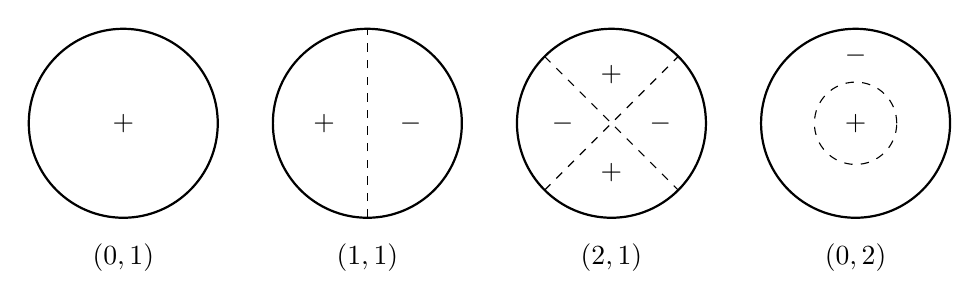
\begin{tikzpicture}
% Mode (0,1)
\begin{scope}
	\draw[thick] (0,0) circle (1.2);
	\node at (0,0) {$+$};
	\node at (0,-1.7) {$(0,1)$};
\end{scope}
% Mode (1,1)
\begin{scope}[xshift=3.1cm]
	\draw[thick] (0,0) circle (1.2);
	\draw[dashed] (0,-1.2) -- (0,1.2);
	\node at (-0.55,0) {$+$};
	\node at (0.55,0) {$-$};
	\node at (0,-1.7) {$(1,1)$};
\end{scope}
% Mode (2,1)
\begin{scope}[xshift=6.2cm]
	\draw[thick] (0,0) circle (1.2);
	\draw[dashed] (-0.849,-0.849) -- (0.849,0.849);
	\draw[dashed] (-0.849,0.849) -- (0.849,-0.849);
	\node at (0,0.62) {$+$};
	\node at (0,-0.62) {$+$};
	\node at (-0.62,0) {$-$};
	\node at (0.62,0) {$-$};
	\node at (0,-1.7) {$(2,1)$};
\end{scope}
% Mode (0,2)
\begin{scope}[xshift=9.3cm]
	\draw[thick] (0,0) circle (1.2);
	\draw[dashed] (0,0) circle (0.523);
	\node at (0,0) {$+$};
	\node at (0,0.86) {$-$};
	\node at (0,-1.7) {$(0,2)$};
\end{scope}
\end{tikzpicture}
\caption{Die vier tiefsten Schwingungsmoden der kreisförmigen Membran.
Der erste Index $n$ zählt die Knotendurchmesser und stammt aus dem Winkelanteil $\cos n\varphi$, der zweite Index $m$ nummeriert die Nullstelle $j_{n,m}$ und bestimmt die Zahl der Knotenkreise im Innern.
Die gestrichelten Linien sind die Knotenlinien, die Vorzeichen geben die Phase der Auslenkung an.
Der innere Knotenkreis der Mode $(0,2)$ liegt bei $j_{0,1}/j_{0,2}\approx 0.436$ des Radius.
Die Frequenzen verhalten sich nach \eqref{bessel:eigenschaften:eqn:eigenfrequenzen} wie $1 : 1.593 : 2.136 : 2.295$.
\label{bessel:eigenschaften:fig:moden}}
\end{figure}
 
%
% Orthogonalität
%
\subsection{Orthogonalität
\label{bessel:eigenschaften:subsection:orthogonalitaet}}
Wie die trigonometrischen Funktionen bilden auch die Bessel-Funktionen ein Orthogonalsystem, allerdings mit einer Gewichtsfunktion.
 
\begin{satz}
\label{bessel:eigenschaften:satz:orthogonalitaet}
Sind $j_{\nu,m}$ und $j_{\nu,l}$ Nullstellen von $J_\nu$, so gilt
\begin{equation}
\int_0^1
J_\nu(j_{\nu,m}s)\,
J_\nu(j_{\nu,l}s)\,
s\,ds
=
\begin{cases}
0 & \text{für } m\ne l,\\[3pt]
\dfrac{1}{2}\,J_{\nu+1}(j_{\nu,m})^2 & \text{für } m=l.
\end{cases}
\label{bessel:eigenschaften:eqn:orthogonalitaet}
\end{equation}
\end{satz}

\begin{proof}
Wir schreiben $\alpha=j_{\nu,m}$ und $\beta=j_{\nu,l}$ sowie $u(s)=J_\nu(\alpha s)$ und $v(s)=J_\nu(\beta s)$.
Setzt man $x=\alpha s$ in~\eqref{bessel:loesung:eqn:bessel} ein und dividiert durch $s$, so erhält man wegen $su''+u'=(su')'$ die selbstadjungierte Form
\begin{equation}
(s\,u')'
+
\Bigl(\alpha^2 s - \frac{\nu^2}{s}\Bigr) u
=
0,
\label{bessel:eigenschaften:eqn:selbstadjungiert}
\end{equation}
und entsprechend für $v$ mit $\beta$ anstelle von $\alpha$.

Multipliziert man~\eqref{bessel:eigenschaften:eqn:selbstadjungiert} mit $v$, die Gleichung für $v$ mit $u$ und subtrahiert, so heben sich die Terme mit $\nu^2/s$ weg und es bleibt
\[
v\,(s\,u')' - u\,(s\,v')'
+
(\alpha^2-\beta^2)\,s\,uv
=
0 .
\]
Der erste Teil ist eine vollständige Ableitung, denn es gilt
$v(su')'-u(sv')' = \frac{d}{ds}\bigl[s(u'v-uv')\bigr]$.
Integration über $[0,1]$ liefert deshalb
\[
\Bigl[\,s\bigl(u'(s)v(s)-u(s)v'(s)\bigr)\Bigr]_0^1
+
(\alpha^2-\beta^2)
\int_0^1 s\,u(s)v(s)\,ds
=
0 .
\]
Am unteren Rand verschwindet die Klammer.
Für $\nu>0$ verschwinden $u$ und $v$ nach~\eqref{bessel:loesung:eqn:kleinx} bei $s=0$ wie $s^{\nu}$ und ihre Ableitungen wie $s^{\nu-1}$, der ganze Ausdruck ist daher von der Ordnung $s^{2\nu}$.
Für $\nu=0$ sind $u$ und $v$ bei $s=0$ beschränkt, und nach~\eqref{bessel:eigenschaften:eqn:j0strich} verschwinden $u'$ und $v'$ dort wie $s$, der Ausdruck ist daher von der Ordnung $s^2$.
Am oberen Rand verschwindet sie, weil $\alpha$ und $\beta$ Nullstellen von $J_\nu$ sind und damit $u(1)=v(1)=0$ gilt.
Für $m\ne l$ ist $\alpha^2\ne\beta^2$, und es folgt die behauptete Orthogonalität.

Für $m=l$ multiplizieren wir~\eqref{bessel:eigenschaften:eqn:selbstadjungiert} mit $2su'$ und erhalten
\[
\frac{d}{ds}\bigl[(s\,u')^2\bigr]
+
(\alpha^2s^2-\nu^2)\,\frac{d}{ds}\bigl[u^2\bigr]
=
0 .
\]
Integration über $[0,1]$ und partielle Integration des zweiten Terms ergeben
\[
2\alpha^2
\int_0^1 s\,u(s)^2\,ds
=
\Bigl[\,(s\,u')^2 + (\alpha^2s^2-\nu^2)u^2\,\Bigr]_0^1 .
\]
Am unteren Rand verschwinden beide Summanden wieder, für $\nu>0$ mit der Ordnung $s^{2\nu}$ und für $\nu=0$ mit der Ordnung $s^2$.
Mit $u'(1)=\alpha J_\nu'(\alpha)$ bleibt
\[
\int_0^1 s\,J_\nu(\alpha s)^2\,ds
=
\frac{1}{2}\,J_\nu'(\alpha)^2 .
\]
Schliesslich ist $J_\nu(\alpha)=0$, aus~\eqref{bessel:eigenschaften:eqn:dreiterm} folgt deshalb $J_{\nu-1}(\alpha)=-J_{\nu+1}(\alpha)$, und~\eqref{bessel:eigenschaften:eqn:ableitungrek} liefert
\[
2J_\nu'(\alpha)
=
J_{\nu-1}(\alpha)-J_{\nu+1}(\alpha)
=
-2J_{\nu+1}(\alpha).
\]
Einsetzen ergibt die behauptete Normierung.
\end{proof}
 
Das Gewicht $s$ im Integral ist kein Schönheitsfehler, sondern das Flächenelement der Polarkoordinaten, $dA = r\,dr\,d\varphi$.
Die Orthogonalität ist also die natürliche Orthogonalität auf der Kreisscheibe.
 
Daraus ergibt sich die \emph{Fourier-Bessel-Reihe}.
\index{Fourier-Bessel-Reihe}%
Eine auf $[0,1]$ hinreichend gutartige Funktion $f$ lässt sich als
\begin{equation}
f(s)
=
\sum_{m=1}^{\infty}
c_m J_\nu(j_{\nu,m}s),
\qquad
c_m
=
\frac{2}{J_{\nu+1}(j_{\nu,m})^2}
\int_0^1 f(s)\,J_\nu(j_{\nu,m}s)\,s\,ds,
\label{bessel:eigenschaften:eqn:fourierbessel}
\end{equation}
entwickeln.
Damit lassen sich Anfangsbedingungen einer kreisförmigen Membran nach Eigenmoden zerlegen, genau wie eine Fourier-Reihe das für die Saite leistet.
 
%
% Asymptotisches Verhalten
%
\subsection{Asymptotisches Verhalten
\label{bessel:eigenschaften:subsection:asymptotik}}
Für grosse Argumente werden die Bessel-Funktionen fast zu trigonometrischen Funktionen.
 
\begin{satz}
\label{bessel:eigenschaften:satz:asymptotik}
Für $x\to\infty$ gilt
\begin{align}
J_\nu(x)
&=
\sqrt{\frac{2}{\pi x}}
\cos\Bigl(x-\frac{\nu\pi}{2}-\frac{\pi}{4}\Bigr)
+
O(x^{-3/2}),
\label{bessel:eigenschaften:eqn:asymptotikj}
\\
Y_\nu(x)
&=
\sqrt{\frac{2}{\pi x}}
\sin\Bigl(x-\frac{\nu\pi}{2}-\frac{\pi}{4}\Bigr)
+
O(x^{-3/2}).
\label{bessel:eigenschaften:eqn:asymptotiky}
\end{align}
\end{satz}

Die im Beweis von Satz~\ref{bessel:eigenschaften:satz:nullstellen} hergeleitete Normalform~\eqref{bessel:eigenschaften:eqn:normalform} macht diese Aussage verständlich.
Der Störterm $(\frac14-\nu^2)/x^2$ verschwindet für $x\to\infty$, und übrig bleibt die gewöhnliche Schwingungsgleichung $u''+u=0$.
Die Lösung ist also asymptotisch eine Schwingung der Kreisfrequenz eins, und der Faktor $1/\sqrt{x}$ kommt von der Rücksubstitution $y=x^{-1/2}u$.

Dieses Argument liefert die Gestalt der Asymptotik, aber nicht die beiden Konstanten.
Sie lassen sich an einem Sonderfall ablesen.
Für $\nu=\frac12$ ist $\frac14-\nu^2=0$, die Normalform lautet dann exakt $u''+u=0$, und die Asymptotik ist keine Näherung mehr, sondern eine Identität.
Tatsächlich gilt
\begin{equation}
J_{1/2}(x)
=
\sqrt{\frac{2}{\pi x}}\,\sin x ,
\label{bessel:eigenschaften:eqn:jhalb}
\end{equation}
wie man durch Einsetzen von $\nu=\frac12$ in die Reihe~\eqref{bessel:loesung:eqn:jnu} und Vergleich mit der Sinusreihe bestätigt.
Setzt man $\nu=\frac12$ in~\eqref{bessel:eigenschaften:eqn:asymptotikj} ein, so ist das Phasenargument $x-\frac{\pi}{4}-\frac{\pi}{4}=x-\frac{\pi}{2}$, und wegen $\cos(x-\frac{\pi}{2})=\sin x$ stimmt die Formel exakt mit~\eqref{bessel:eigenschaften:eqn:jhalb} überein.
Damit sind sowohl die Amplitude $\sqrt{2/\pi}$ als auch der Phasenanteil $-\pi/4$ festgelegt.

Der verbleibende Phasenanteil $-\nu\pi/2$ lässt sich ebenfalls kontrollieren.
Leitet man die Asymptotik von $x^{-\nu}J_\nu$ ab und vergleicht mit~\eqref{bessel:eigenschaften:eqn:ableitung2}, so verschiebt jeder Schritt von $\nu$ auf $\nu+1$ die Phase um genau $\pi/2$.
Ein vollständiger Beweis für beliebiges $\nu$ verlangt eine echte asymptotische Analyse.
Für ganzzahliges $\nu=n$ leistet das die Methode der stationären Phase, angewandt auf die Integraldarstellung~\eqref{bessel:eigenschaften:eqn:integral}, für allgemeines $\nu$ braucht man eine Integraldarstellung, die auch für nicht ganzzahlige Ordnung gilt.
Die Einzelheiten finden sich bei \cite{bessel:watson} und \cite{bessel:dlmf}.

Die Lösung ist also asymptotisch eine Schwingung, und der Faktor $1/\sqrt{x}$ kommt von der Rücksubstitution.
 
Die Abklingrate $1/\sqrt{x}$ ist physikalisch einleuchtend.
Eine von einem Punkt ausgehende Kreiswelle verteilt ihre Energie auf einen Kreis mit Umfang $2\pi r$, die Energiedichte fällt also wie $1/r$ und die Amplitude wie $1/\sqrt{r}$.
Wirft man einen Stein ins Wasser, sieht man genau das.
 
Zusammen mit~\eqref{bessel:loesung:eqn:kleinx} ist das Verhalten von $J_\nu$ damit in beiden Grenzfällen bekannt.
Nahe null verhält es sich wie eine Potenz $x^\nu$, weit draussen wie eine gedämpfte Kosinusschwingung.
Der Bereich dazwischen ist der interessante, und dort hilft nur die Reihe oder die Numerik.

 
\printbibliography[heading=subbibliography]
\end{refsection}
 
%
% Notizen aus der ersten Planungsphase (nicht löschen, bis alles
% eingearbeitet ist, dient als Kontrollliste)
%
% - Wie findet man die Gleichung?            -> teil1
% - Warum keine gewöhnliche Potenzreihe?     -> teil2, Anschluss an
%                                               Abschnitt "Fuchssche
%                                               Differentialgleichung"
% - Welche Phänomene, woher kommt die DGL?   -> teil1 (Membran),
%                                               teil5 (Optik),
%                                               teil6 (Himmelsmechanik)
% - Wie löst man eine DGL mit Potenzreihen?  -> steht schon im Buch,
%                                               nur referenzieren
% - Rotationssymmetrie als roter Faden       -> teil1 und teil0
% - "Braucht einen Trick" = verallgemeinerte
%   Potenzreihe mit Exponent varrho          -> teil2
%